\documentclass[12 pt]{article}

\usepackage{hyperref}
\usepackage{pdfpages}
\title{May 2015 Work Log}

\author{Jeremy Rogers \\
	\texttt{jroger44@vols.utk.edu}}

\date{May, 2015}
\begin{document}
	\maketitle
	
	\tableofcontents
	
	\section{Goals for the Month}
	\begin{enumerate}
		\item Install \LaTeX\ for these notes
		\item Get access to the repository and Gauley
		\item Read through all of Logan's previous notes
		\item Brush up on R by looking through the user manual
		\item Begin looking through the code on the repository
		\item Create a repository for these notes
		\item Get a Linux install working on my machine
		\item Read up on MCMC
		\item Begin running Logan's old code
		\item Create my own genome for testing
		\item Refactor the visualization script
		\item Set up the printer for timesheets
	\end{enumerate}
	
	\section{Progress/Notes}
	
	\subsection{Install \LaTeX\ for these notes}
		\begin{enumerate}
			\item \LaTeX\ has been installed and tested
		\end{enumerate}
	
	\subsection{Get access to the repository and Gauley}
		 \begin{enumerate}
		 	\item With Dr. Gilchrist, I was able to get access to both repositories (the one with Logan's notes and the one containing CUBfits). I also was granted an account on Gauley and Newton.
		 \end{enumerate}
	\subsection{Read through all of Logan's previous notes} 
		\begin{enumerate}
			\item I should check out his script repository later, when I need to begin testing this. He says it's located at \url{https://github.com/ozway/cubmisc}
			\item After reading through all the notes, it appears that his code is close to completion. There are a few things that he mentioned wanting to do, and I'm not sure if he got around to those.
			\item He mentions moving some of the code to C from R, but he feels that it would be more work than it is worth.
			\item He also mentions debugging the genome creation process by using a genome that is totally dominated by mutation bias, and see if the genome is correctly created across all phi values.
			\item He also mentions changing some divisions to subtractions using logarithm rules, since that would be quicker.
			
			\item Just some terminology that I need to remember:
			\begin{enumerate}
				\item CUB -- codon usage bias
				\item $ \eta $ -- cost-benefit ratio of protein synthesis
				\item $ \phi $ -- protein synthesis rate
				\item $ N_e $ -- population size
				\item ROC -- ribosome overhead costs
				\item NSE -- nonsense error
				\item ORFs -- Open Reading Frames
				\item $ q $ -- proportional decline in fitness per ATP wasted per unit time
				\item $ \Delta M $ -- mutation bias
				\item $ E(\phi) $ -- expected protein synthesis rate, should be 1 if time units are defined correctly
				
			\end{enumerate} 
		\end{enumerate}
		
		\subsection{Read the R Manual}
		\begin{enumerate}
			\item I have read the first 3 chapters. I feel like I have a good grasp on the R language and environment now.
		\end{enumerate}
		
		\subsection{Read through the code on the repository}
			\begin{enumerate}
				\item I have begun to read through the main staples of the code (namely \texttt{my.cubappr.r} and \texttt{roc.appr.r}). This is a lot of code, in a language that I've only used in passing, so it could take a while to figure this out. 
			\end{enumerate}

		
		\subsection{Create a repository for these notes}
			\begin{enumerate}
				\item Repository has been created at \url{https://github.com/jeremyrogers/EEB}
			\end{enumerate}
			
		\subsection{Get a Linux Install working on my machine}
			\begin{enumerate}
				\item This is a low priority, but I'd still like to get it done by the end of the week. According to the documentation on \texttt{CUBfits}, some of the parallel stuff might bug out on Windows.
				\item May 13 Update: I have a working linux install now, so that will dramatically help to test these things.
			\end{enumerate}
			
		\subsection{Read up on MCMC}
			\begin{enumerate}
				\item Thanks to Stack Exchange's math section, I found a really nice explanation on MCMC. After reading that, I was able to parse through the rather technical Wikipedia page on the subject, and now I feel like I have a good grasp on this.
			\end{enumerate}
		
		\subsection{Run Logan's code}
			\begin{enumerate}
				\item Logan's code from his \texttt{cubmisc} repository was pretty broken on my machine, but that could have just been my configuration. After fixing the initial errors I received, I began running his \texttt{run\_roc.r} test script at 15:35 on May 13. I left at 17:35 and it was still running on Gauley.
				\item The next morning at 10:55 when I got in, it had halted execution with this error:
				\begin{verbatim}
				Error in my.set.adaptive(nIter + 1, n.aa = n.aa, 
				b.DrawScale = b.DrawScale,  : 
				length of p.DrawScale is incorrect.
				Calls: system.time ... cubsinglechain -> do.call -> 
				<Anonymous> -> my.set.adaptive
				Execution halted
				\end{verbatim}
				
				I'm not really sure what any of this means, and it's entirely possible that this isn't his final code, being this other repository I found. However, this is currently the best lead I have on which code was Logan's. According to Cedric, there were 1 or 2 functions in the \texttt{cubfits} library that Logan wrote, but we're unsure of which ones they are.
				
				\item I tried to run his \texttt{run\_nsef.r}, but it halted with these errors:
				\begin{verbatim}
					Error in phi.New[accept] <- prop$phi.Prop[accept] : 
					NAs are not allowed in subscripted assignments
					Calls: system.time ... cubsinglechain -> do.call -> 
					<Anonymous> -> my.drawPhiConditionalAll
					In addition: Warning messages:
					1: In dlnorm(phi.Obs, log(phi), sigmaW, log = TRUE) : NaNs produced
					2: In rnorm(1, mean = log.sigma.Phi.Curr, sd = sigma.Phi.DrawScale) :
					NAs produced
					3: In my.drawRestrictHP(proplist, list.Curr, phi.Curr) :
					log acceptance probability not finite in hyperparam draw
					4: In rnorm(1, mean = bias.Phi.Curr, sd = bias.Phi.DrawScale) :
					NAs produced
					5: In my.drawbiasPhi(proplist, list.Curr, log.phi.Obs, log.phi.Curr,  :
					log acceptance probability not finite in hyperparam draw
					Execution halted
				\end{verbatim}
				
				This will be fun.
				
				\item After speaking with Dr. Gilchrist, it is clear that my main objective at the moment is to run the first order approximation of the NSE model on the genomes, both simulated and actual. For the simulated genomes, I must find the values used to see if we can reconstruct them accurately using the first order NSE approximation.
				
				\item I've been tweaking Logan's NSE code to parallelize a little, since his wasn't parallelized at all. Hopefully this will take less time to run now. In order to make it parallel, all I had to do was near the beginning of the code, add \texttt{config\$parallel <- "mclapply"}. I did \texttt{mclapply} since I'm running this on Gauley with shared memory. If I move this to Newton, which I probably will at some point, I'll have to use \texttt{task.pull}
				
				\item I've been tweaking some settings to try to get this to work properly. I had a few different errors that were quick fixes, but this one is a head scratcher. Running the code, I get this error, the same one from before:
				\begin{verbatim}
					running cubappr using cubsinglechain 
					with seeds: 84953
					Running in parallel mode mclapplyError in my.set.adaptive(nIter +
					 1, n.aa = n.aa, b.DrawScale = b.DrawScale,  : 
					length of p.DrawScale is incorrect.
					Calls: system.time ... cubsinglechain -> do.call -> <Anonymous> ->
					 my.set.adaptive
					Timing stopped at: 22.393 4.374 18.18 
					Execution halted
				\end{verbatim}
				
				Length of p.DrawScale is incorrect? I looked at my.adaptive.DrawScale, and found some pertinent lines of code. However, there are 4 places which print the \texttt{length of p.DrawScale is incorrect} error. So, now I have to figure out which one it is.
				
				My first thought was to add print statements in each one to see which one was getting triggered. I did that, but there were problems building it locally on Gauley. First, \LaTeX\ wasn't installed, and for some reason, that caused the build to fail. So I got Cedric to install \texttt{texlive} for me. Once that was installed, it built properly. However, when I would try to run it with the local library, R couldn't find it. Maybe I just don't know enough about R. I'll look into that later. 
				
				Cedric mentioned using R's \texttt{browser()} function to figure out where I am in the code. I'll begin looking through the R manual to learn that function.
				
				I've narrowed it down significantly now. Logan's \texttt{run\_roc.r} calls a function called \texttt{cubsinglechain}. I used \texttt{grep} to find it in the \texttt{cubfits} source, and it's in the file \texttt{cedric.convergence.r}. From there, it appears that it's in line 221, which has \texttt{res <- do.call(cubfits, c(input\_list, list(phi.Init = init.phi), list(p.Init = p.init), list(b.RInit = b.rinit), list(b.Init = b.init),
					list(b.DrawScale = b.DrawScale), list(p.DrawScale = p.DrawScale), list(phi.DrawScale = phi.DrawScale)))
					} 
					
				I'm unsure of what's going on here for now. I'll ask Cedric at some point.
				
				On May 14, I spent a good part of the day learning how to use custom packages in R, so that I could build this stuff locally to debug and to edit things. 
				
				I decided to try to build \texttt{cubfits} locally, with a print statement after setting \texttt{p.DrawScale}. After adding that, it magically is working now. I began running it at 12:14 on May 17, so I'll see where this goes. 
				
				Maybe this actually works sometimes, and I just got lucky with it working this time after adding a line. Or maybe the version of \texttt{cubfits} I built locally is different than the one I got from \texttt{CRAN}. Regardless, it's still running now at 13:37, so hopefully it will stay this way. For the record, I'm running this with the Brewers' Yeast genome, with the initial phi values given in the same directory.
				
				I've restarted the script now with less samples (750 down from 6000) in order to save some time. I'm also running it with the ecoli genome now, just for a change in testing. I began this run at 14:53 on May 18. 
				
				I checked it at around 21:00, and it had completed! Finally. It created 4 files, \texttt{ecoliwithPhi.bmat}, \texttt{ecoliwithPhi.dat}, \texttt{ecoliwithPhi.log}, and \texttt{ecoliwithPhi.phi}. Now I'll have to figure out what each of these files does, and visualize them.
				
				Obviously, \texttt{ecoliwithPhi.log} is the log file. According to this, the time for 1 chain on 5 cores was 226.63 minutes. It apparently finished at 18:52, which was actually much earlier than I expected. Reducing the samples helped that a lot I would assume.
				
				\texttt{ecoliwithPhi.bmat} has a list of values for proteins and values with standard deviations. I assume the value is the mean for the data set? Not sure.
				
				\texttt{ecoliwithPhi.phi} is a list of ORFs and information about them, such as arithmetic means of $ \phi $, geometric means, \texttt{harm\_mean} (harmonic mean?), and standard deviations. Neat.
				
				\texttt{ecoliwithPhi.dat} is unreadable with a standard text editor. I'm not really sure what it holds.
				
				I found his file \texttt{visualize.r} in the directory. I ran it, but it was broken because the directories and files were hardcoded. I made those customizable at the top, and fixed them to fit my files, and it graphed! I'm not really sure what these graphs mean, but I can figure out some of them. The estimated $ \phi $ vs. observed $ \phi $ graph has an awful correlation coefficient, with $ R^2 = .138 $. That's abysmal, but I feel it could be because I ran it with very few samples. Or maybe it's supposed to be bad.
				
				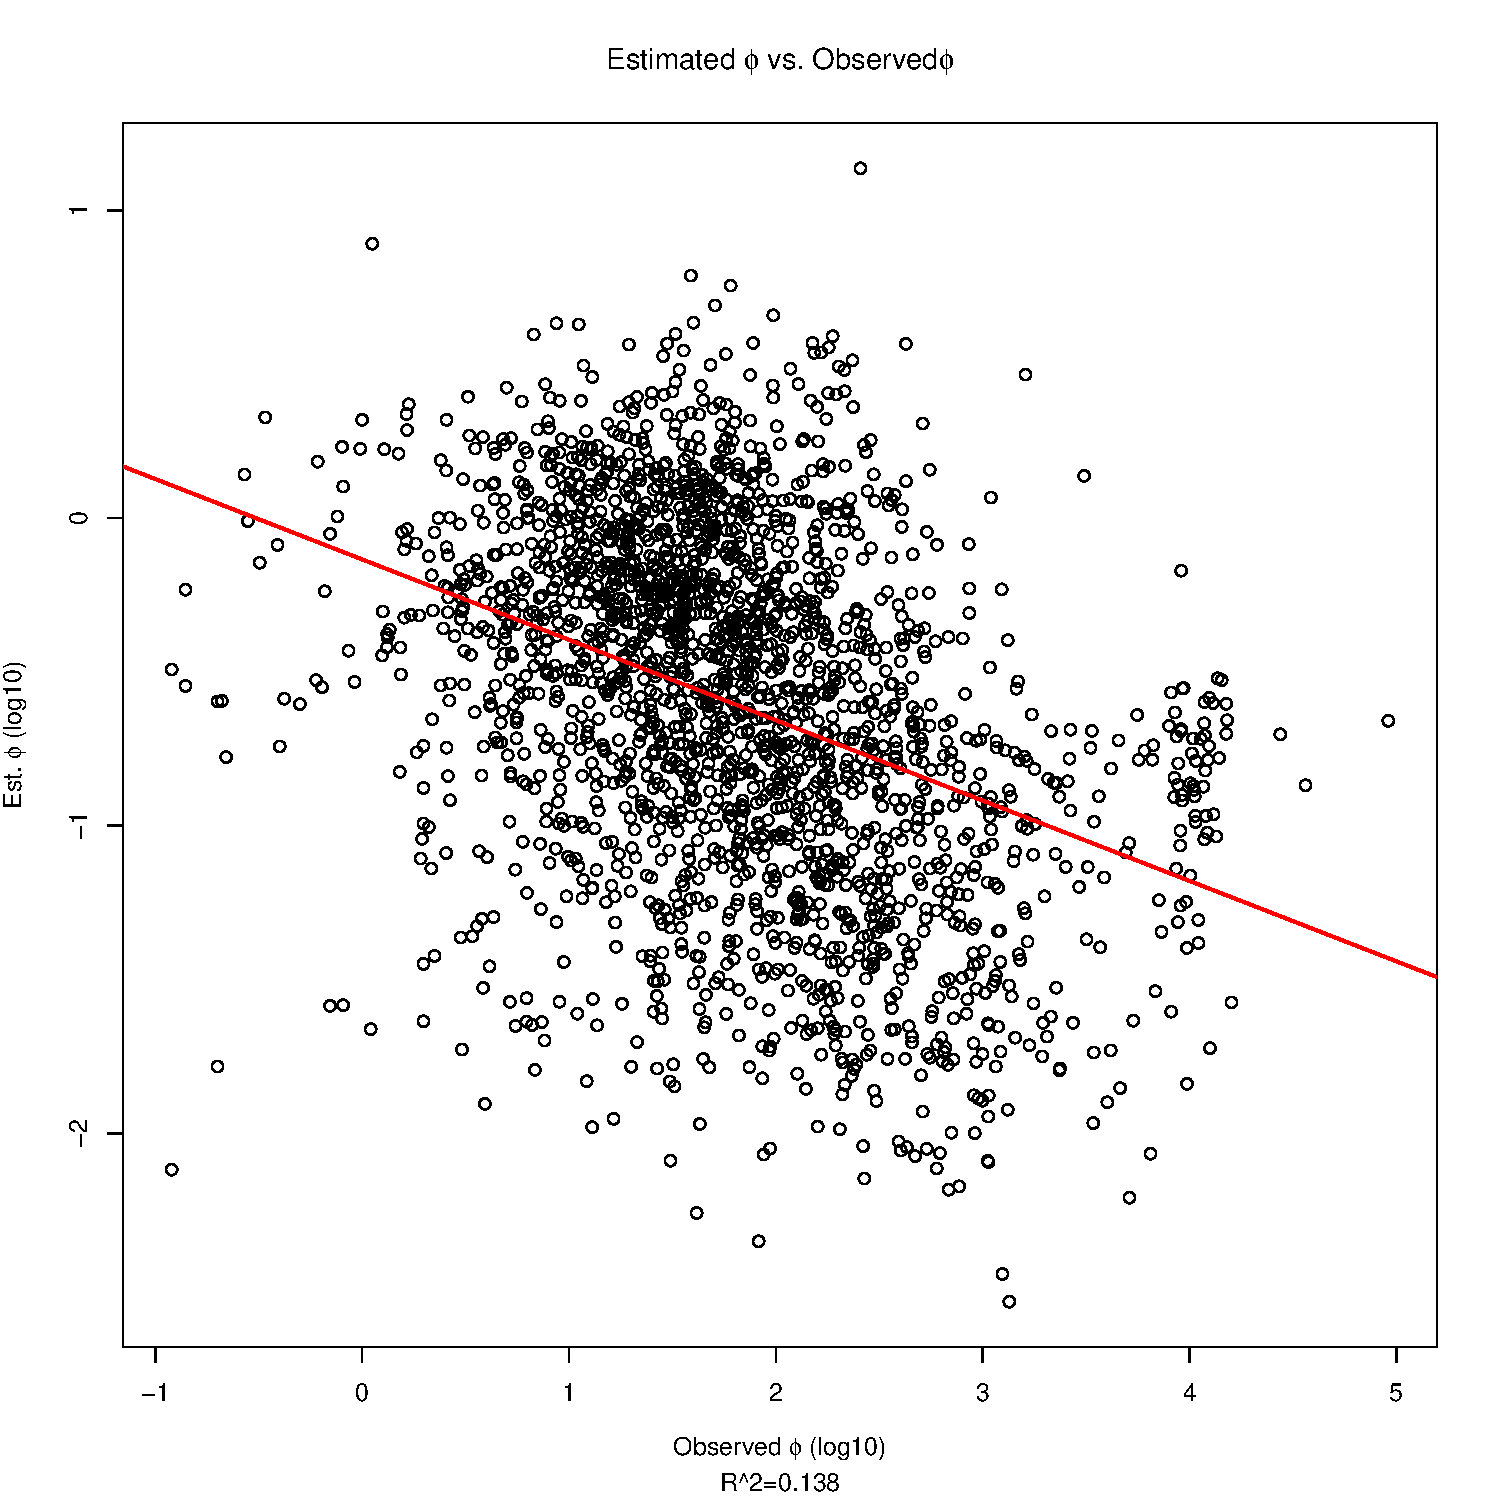
\includepdf{graphs/ecoli/750samples/ecoli_vs_obs_phi_05-19.pdf}
				
				All of the graphs that I got are available in the \texttt{graphs} directory. 
				
				I've begun cleaning up his visualization code, as there's a lot of things hard coded that are hard to edit, so it should be nicer to change up for different genomes now. Also, with his previous code, it only worked for the genomes he was specifically testing. After I edit it, it should work for any given genome.
				
				While working on the visualization script, I've begun running the NSE approximation on the Brewers' Yeast at 15:34. This time, again, with 750 samples for brevity, just to see if it works. It should be done, judging by the time it took the ecoli genome, around 6 or 7.
				
				Well, that took much longer than expected. I'm not sure why it took so much longer on the Brewers' Yeast. I checked it at 19:00 and then again at 22:00, and it was still running. It finally finished at 3:42 the next morning, May 20. It had a runtime of about 721 minutes. I'll ask Cedric why the brewers' yeast took so much longer than the ecoli genome (around a factor of 3 slower).
				
				Regardless, the graphs for this are in the \texttt{graphs} directory as well. Note in the estimated $ \phi $ vs. observed $ \phi $ graph, the correlation coefficient is much better, at $ R^2 = .597 $. That's not great, but it's much better than the ecoli genome's graphs. Perhaps this is related to why the brewers' yeast genome took so much longer.
				
				I talked to Cedric about the discrepancy in times, and he said it's probably attributed to simply the lengths of the genomes. So, I think that's alright.
				
				I began running the 6000 sample version of the ecoli NSE model, and it took a whopping 47 hours to complete. However, looking at the graphs it created, they're not as great as I expected. The estimated $ \phi $ vs. observed $ \phi $ graph, shown below, has a correlation coefficient of .525, worse than the 750 sample run for the Brewers' Yeast. Also shown below are the CUB graphs. Perhaps the initial guesses are bad. I used SCUO for the initial guesses, since that's the way Logan left it. I'll look into some other initial conditions and see if I can improve this.
				
				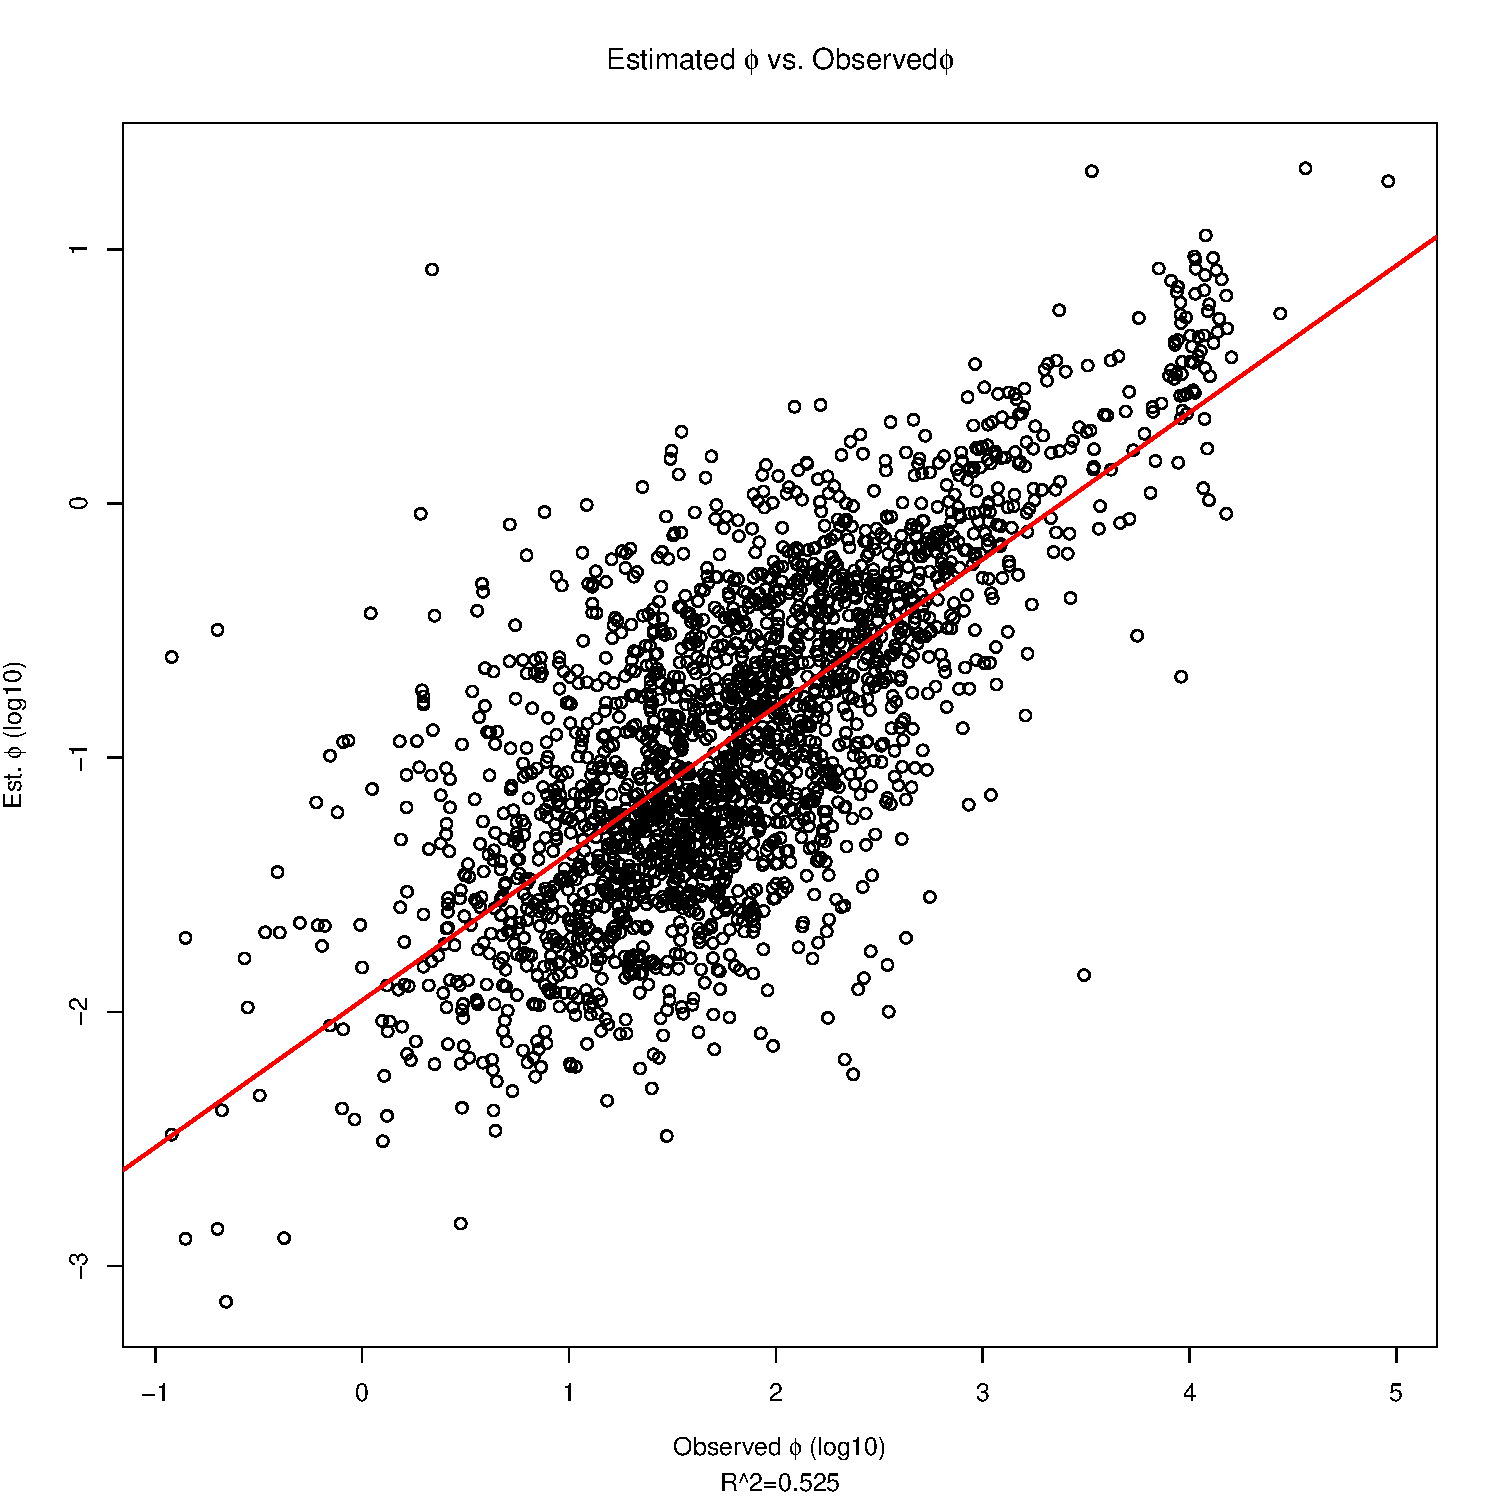
\includepdf{graphs/ecoli/6000samples/6000samplesecoli_vs_obs_phi_05-21.pdf}
				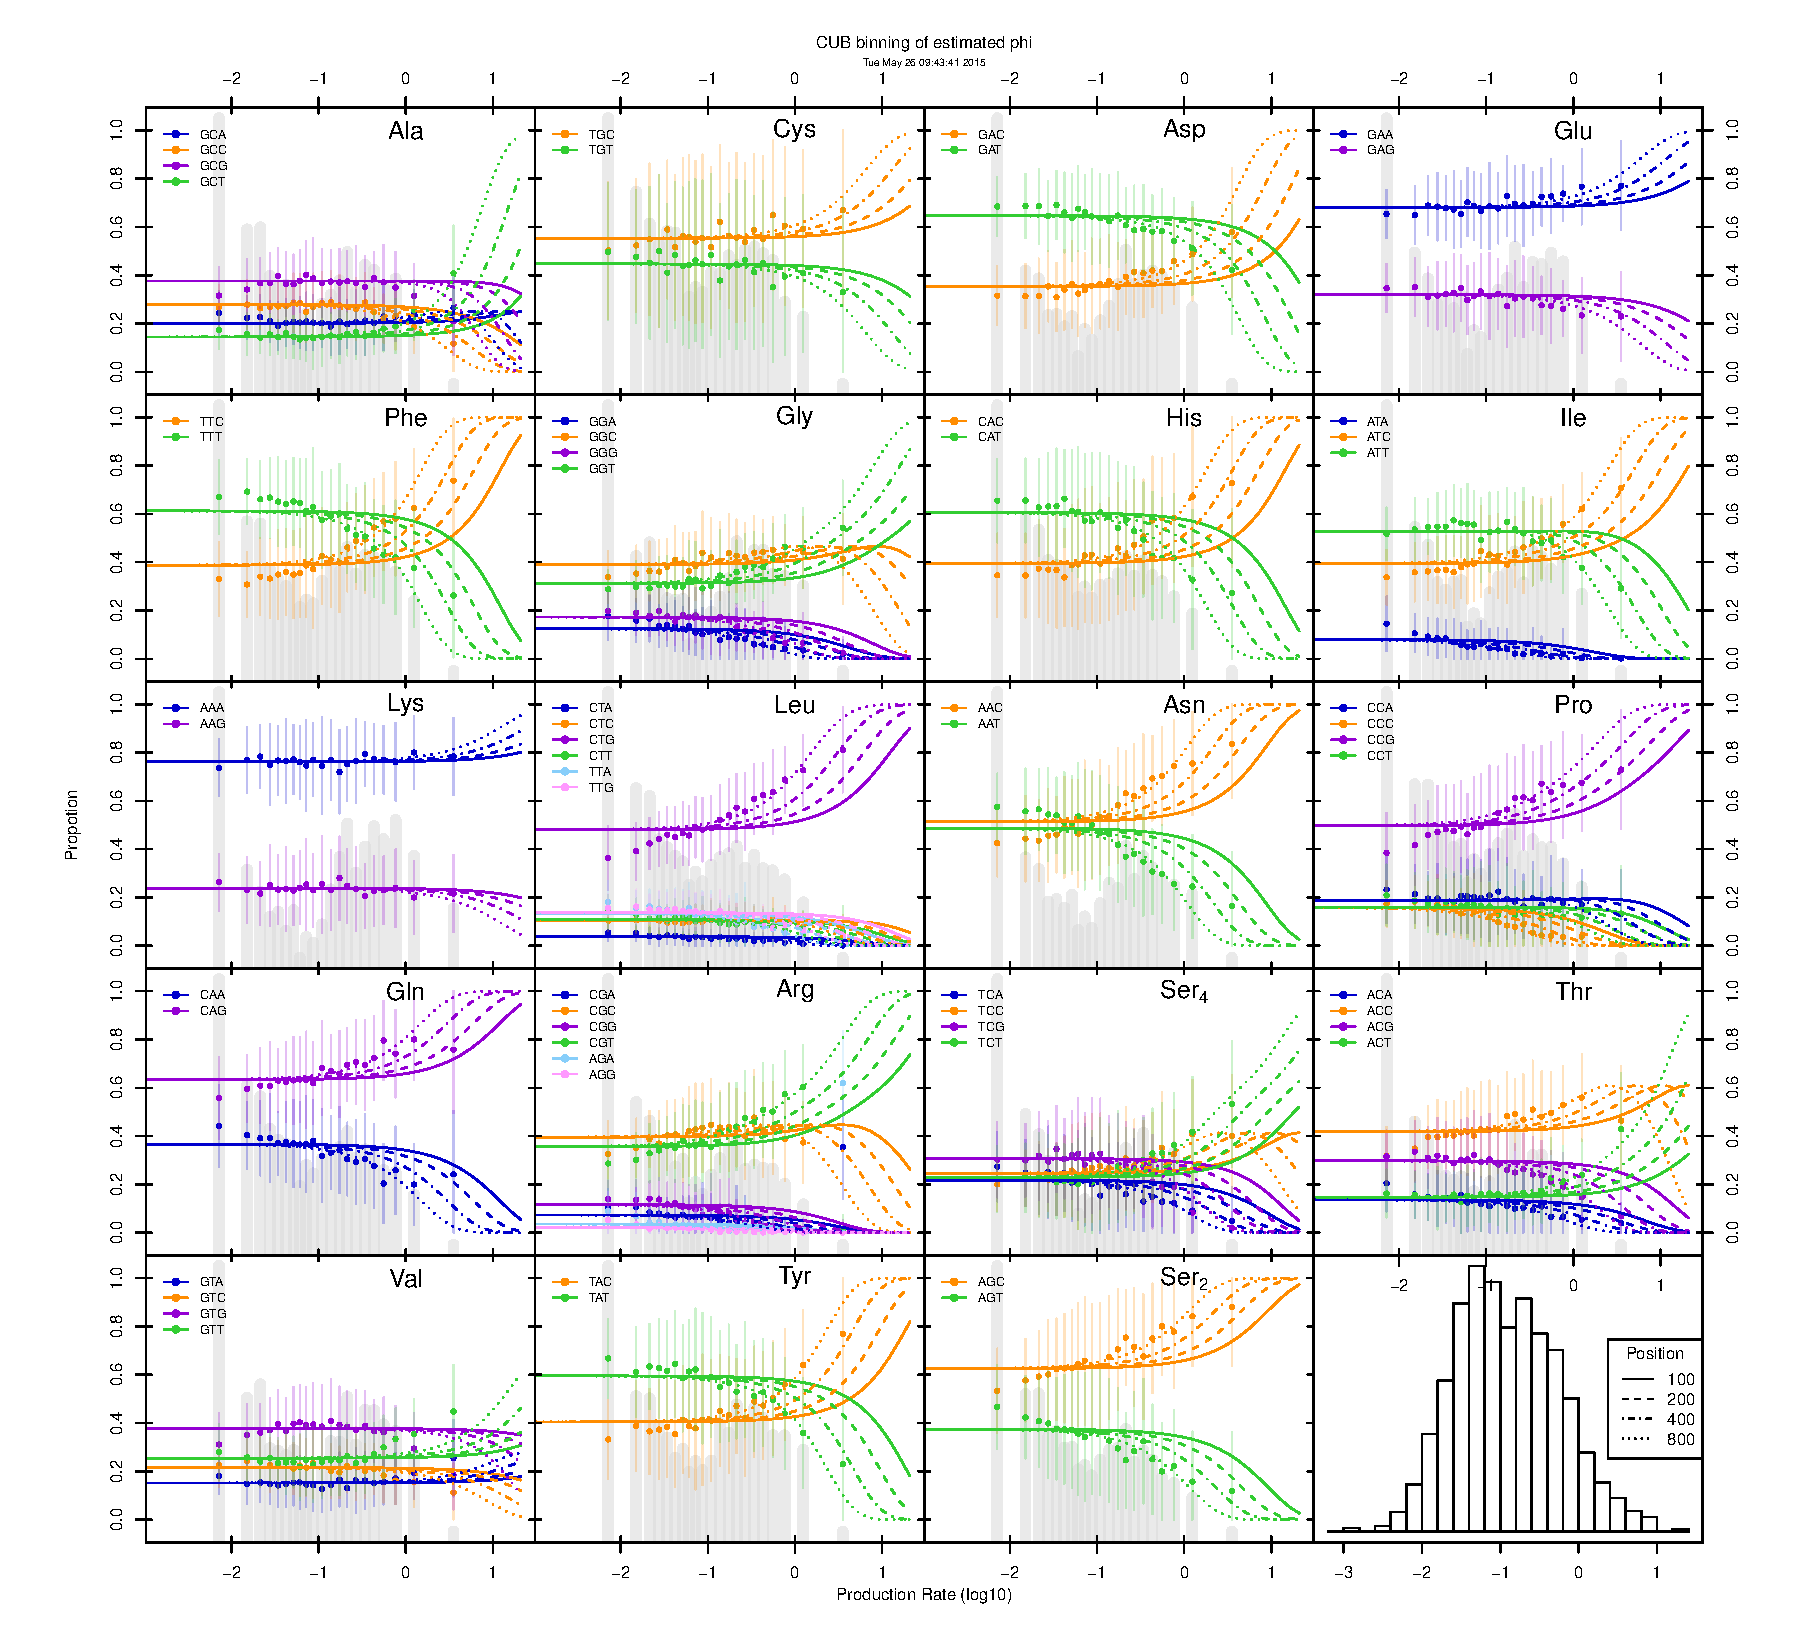
\includepdf{graphs/ecoli/6000samples/6000samplesecoli_CUB_est_bin_05-21.pdf}
				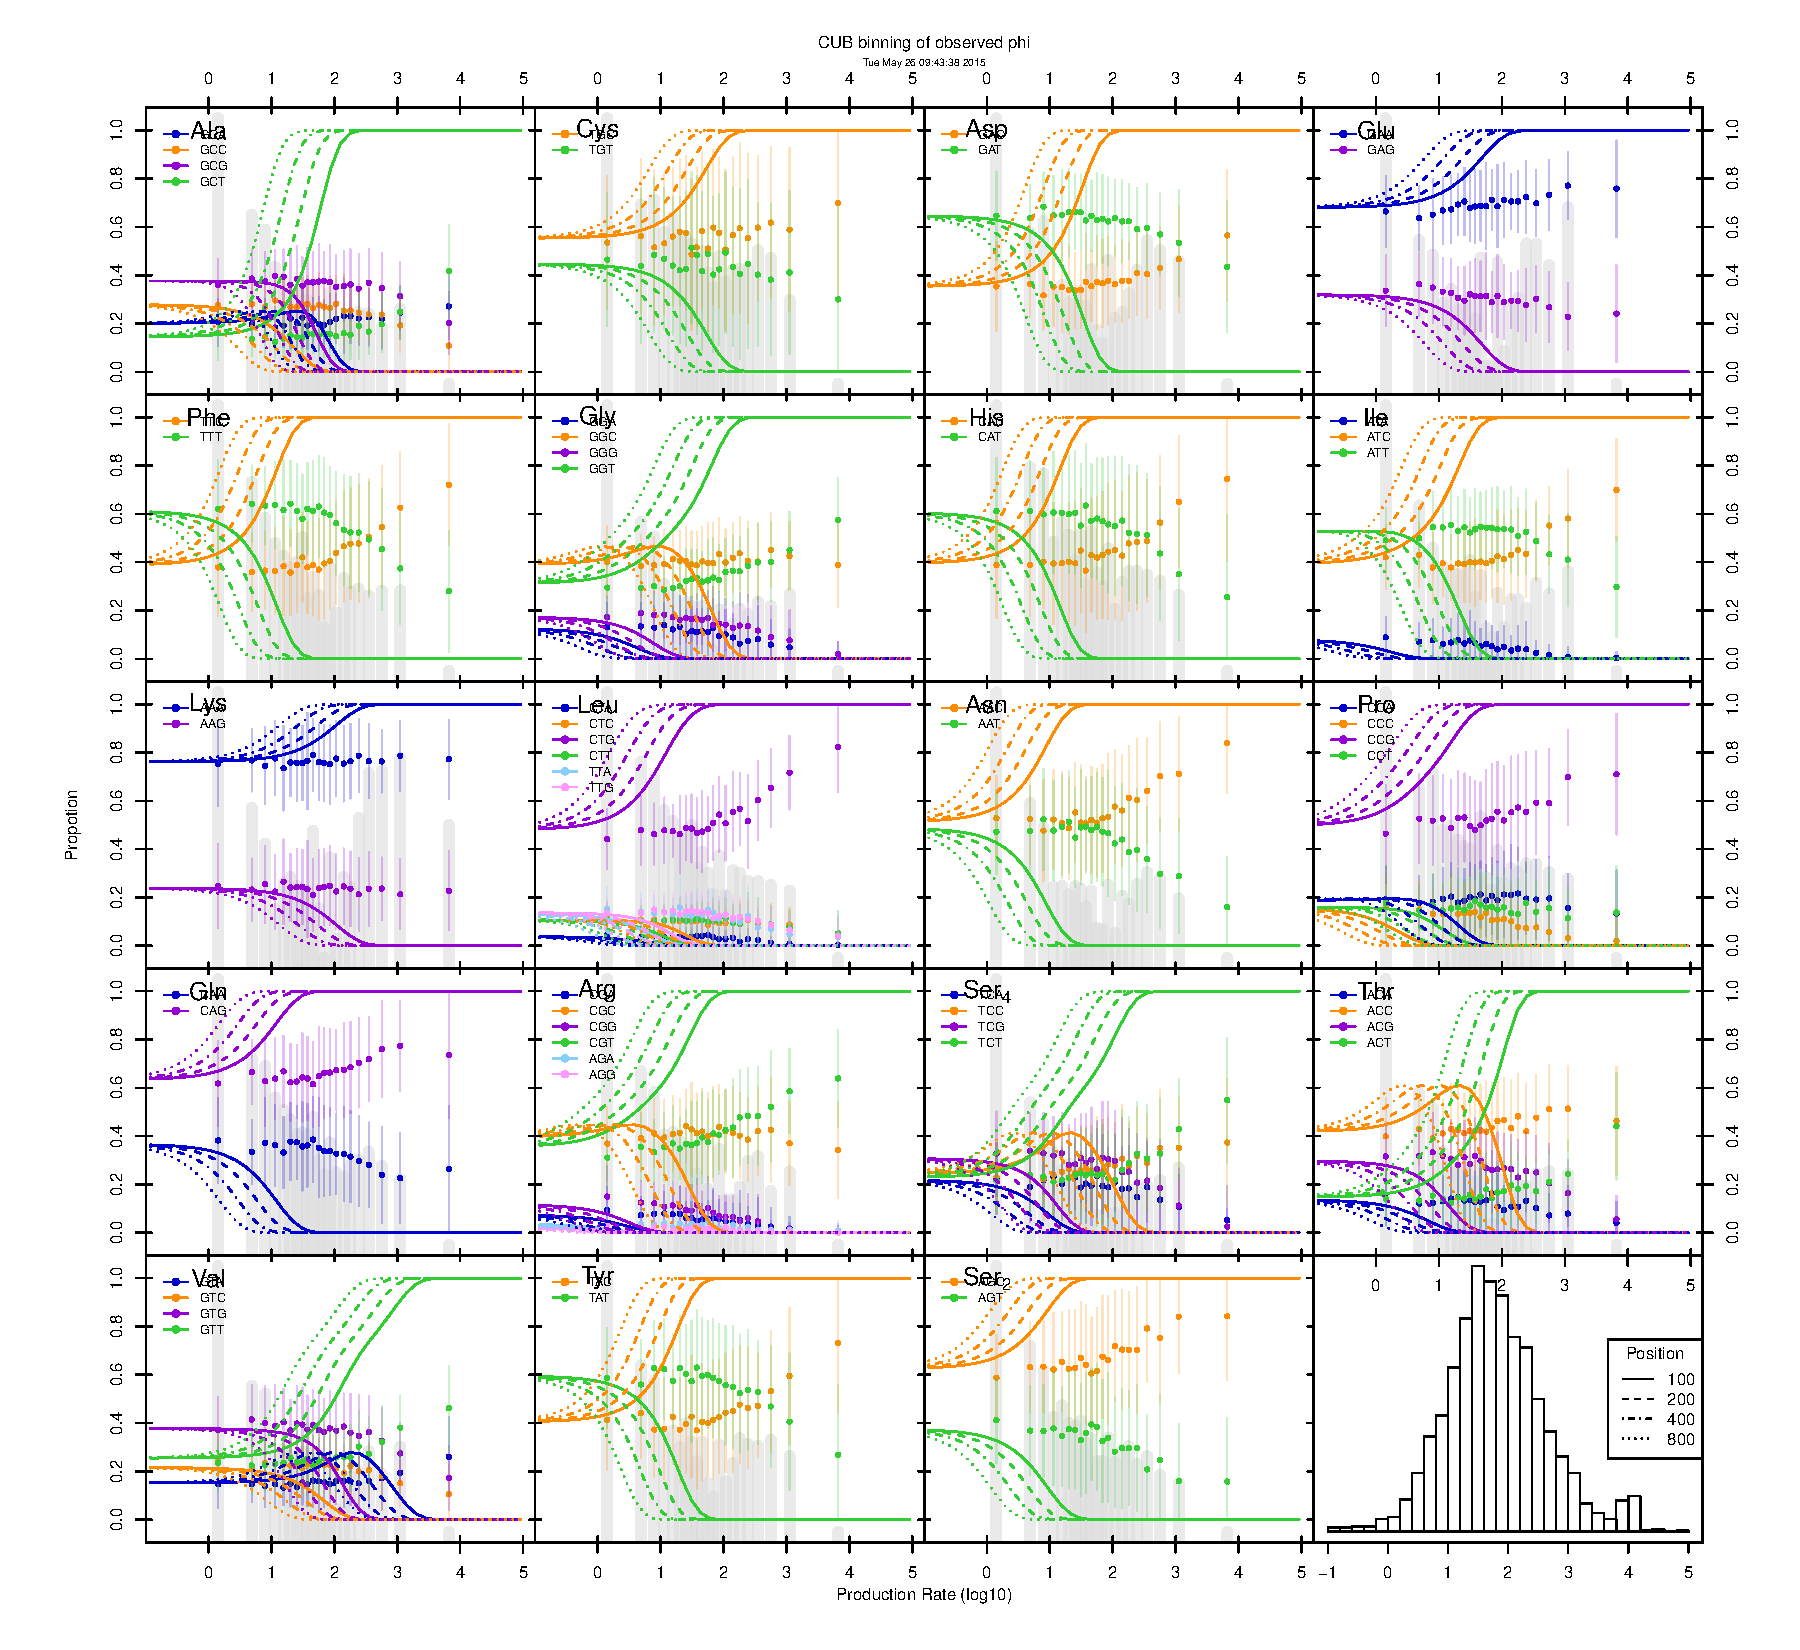
\includepdf{graphs/ecoli/6000samples/6000samplesecoli_CUB_obs_bin_05-21.pdf}
				
				Dr. Gilchrist mentioned changing the proteins to only include the ones that have 2 amino acids. Apparently, the ones that have more than 2 kill performance. Interesting. I'll do that for testing from now on.
				
				After running a few more tests, it seems that the model fits the REU13 yeast closest. This one fits almost perfectly to everything. Maybe if I can figure out why this one fits so well, I can get the others to fit as well. The Brewers' Yeast, Preston's Yeast, and Logan's Yeast aren't necessarily bad, but they're nowhere close to the REU13 yeast. This was run with $ a_1 = a_2 = 4 $, per Logan's request. I'll try different values of $ a_1 $ and $ a_2 $ for the different runs, especially with the ones that are actual genomes, since it's hard to know what $ a_1 $ and $ a_2 $ should actually be.
				
				
 			\end{enumerate} 
 			
 		\subsection{Create my own genome}
 		\begin{enumerate}
 			\item Dr. Gilchrist mentioned creating my own genome, and seeing if the model would accurately recreate the data from the new genome, so I began looking into that.
 			\item In Logan's logs, he mentions creating his own genomes, and that he moved everything to a repository, but he didn't write which repository. With Cedric's help, I found an NSE repository on Gauley that I think contains the right script. It's found (on Gauley) at \\
 			\texttt{/export/home/semppr/gitrepos/clandere/nse.git} for future reference. The repository at \\
 			\texttt{/export/home/semppr/gitrepos/clandere/roc.git} contains most of the meat of this stuff as well.
 			\item I'm having some trouble installing the \texttt{NSEexchange} package to R. After doing the same thing I was doing with \texttt{cubfits}, it doesn't work with the \texttt{NSEexchange}. I can't install it to R on Gauley since I don't have root access on there.
 			\item I finally got the genome sequencing working. For future reference, I needed the dependencies stored at \texttt{/export/home/lbrown/cubfits/Dependencies}. Anyways, I have sequenced Jeremy's Yeast, and I am now running the NSE first order approximation model with 2000 samples on it.
 			\item The run finally finished at 10:06, after about 41.5 hours. I was a little surprised by how long it took, but then again, it was a 2000 sample run, with a rather large genome (around 5000 genes). The results are.... interesting. The $ \phi $ convergence is good, much better than most of the other genomes, at $ R^2 = .688 $. However, the $ \omega $ convergence is laughably bad. Correlation of $ R^2=.000288 $, and the best fit line is a horizontal line. Maybe I used the wrong file for the $ \omega $s or something. I'll look into it.
 			
 			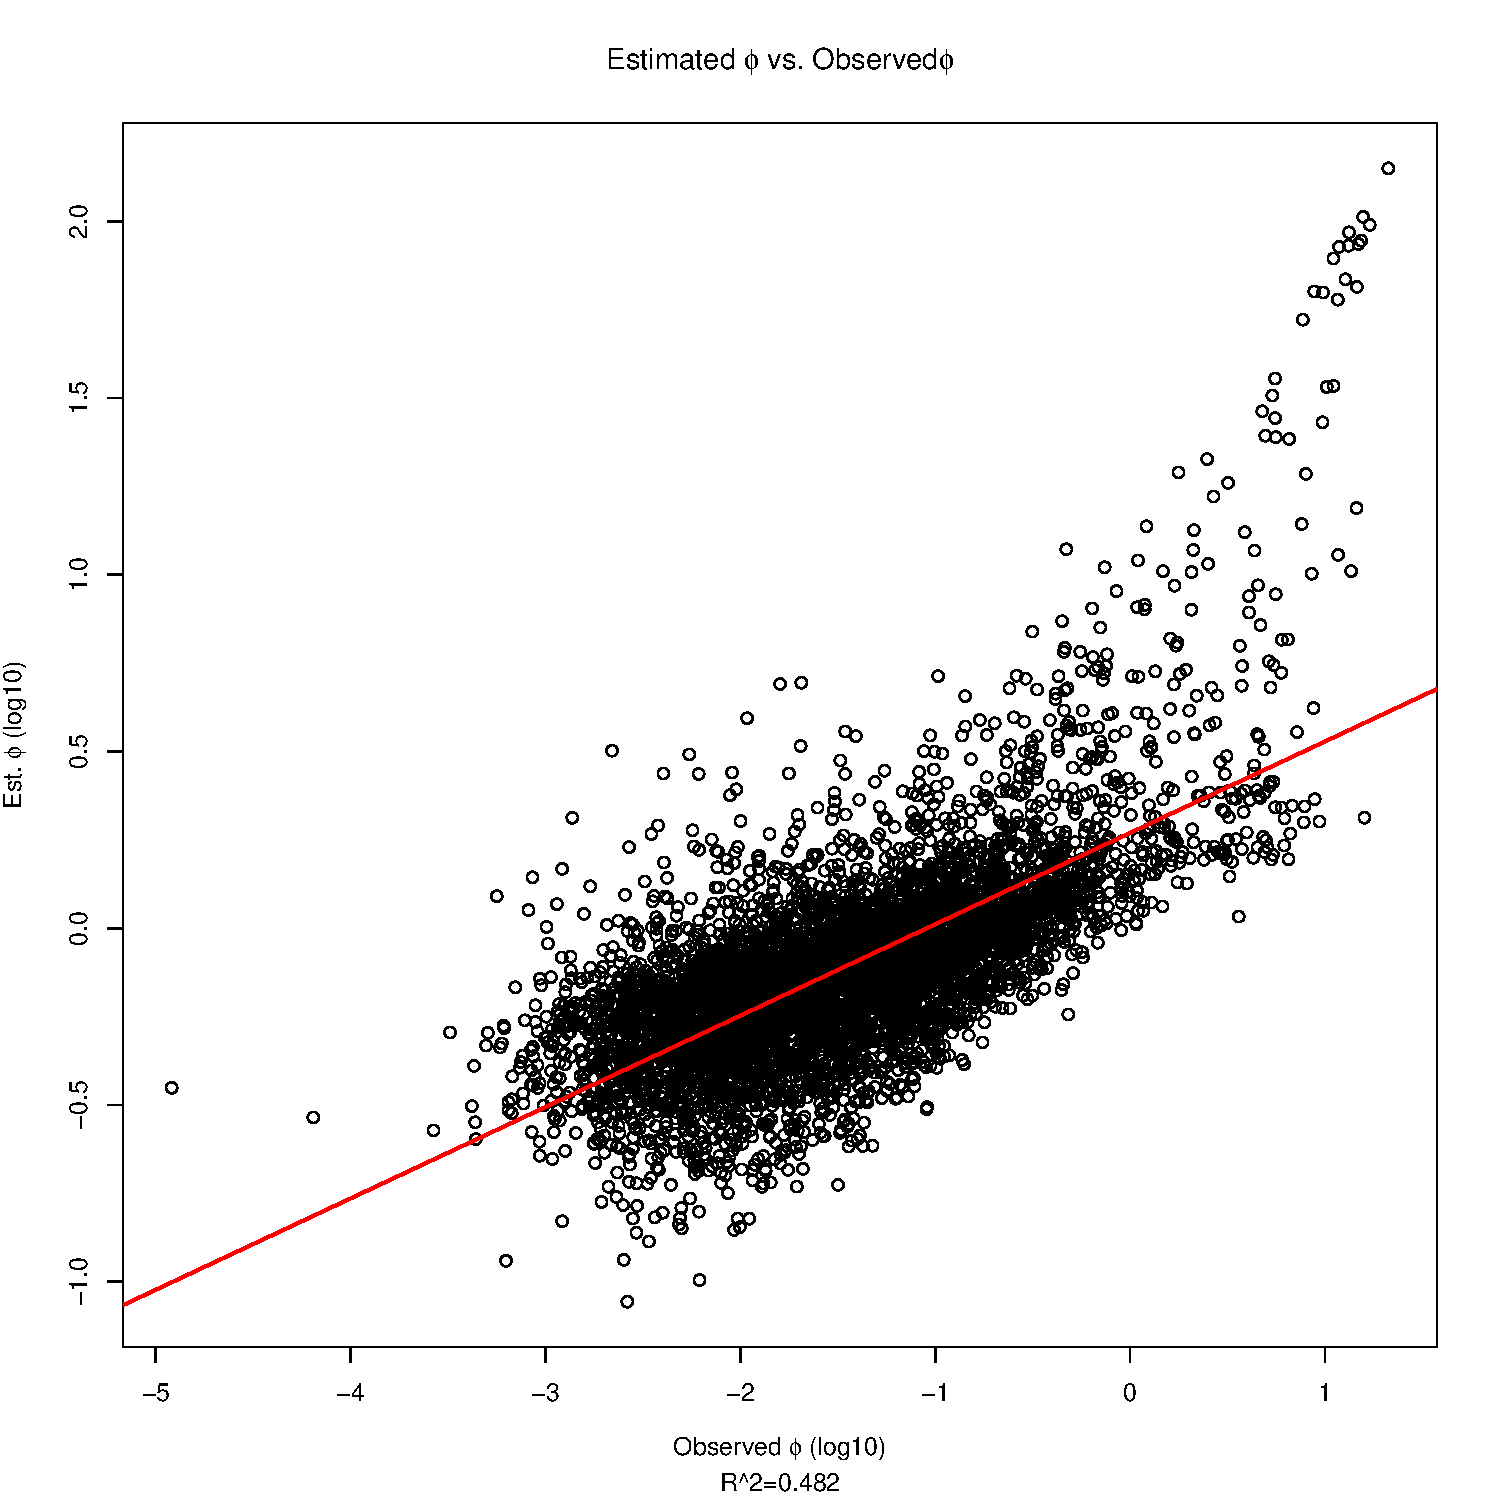
\includepdf{graphs/jeremyyeast/jeremy_vs_obs_phi_05-27.pdf}
 			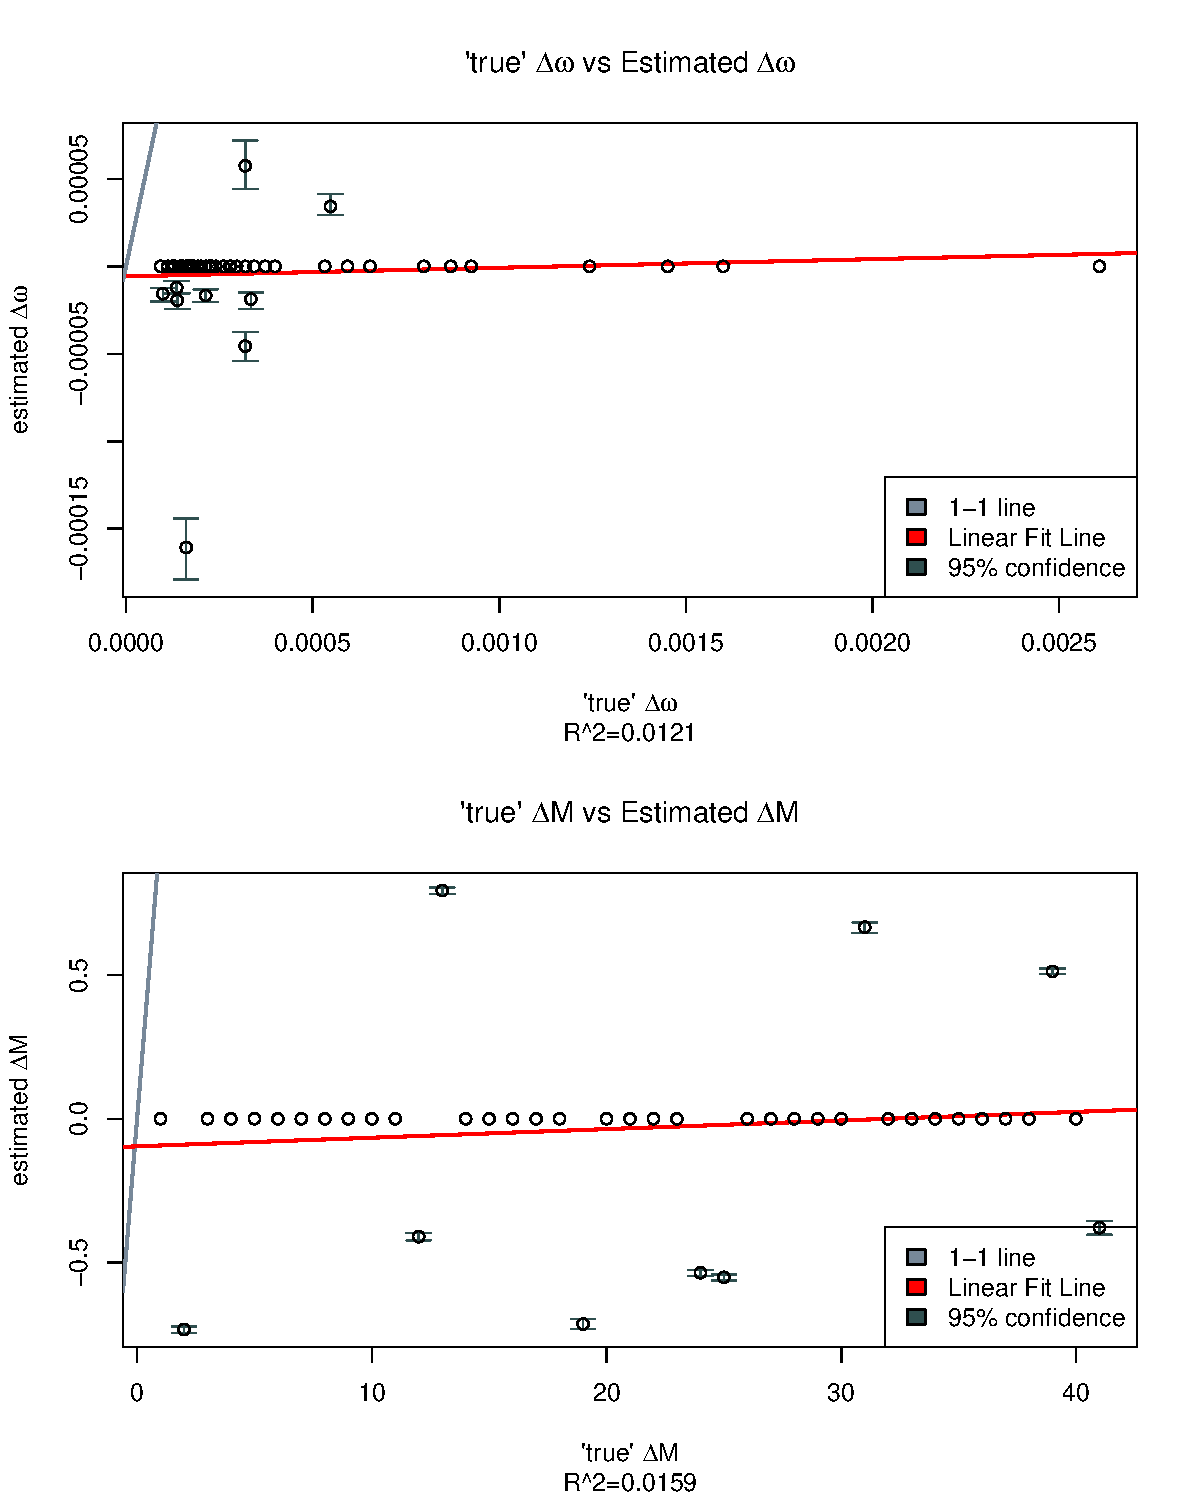
\includepdf{graphs/jeremyyeast/jeremy_codonParameters_05-27.pdf}
 		\end{enumerate}
 		
 		\subsection{Refactor the visualization script}
 		\begin{enumerate}
 			\item Since Logan's visualization script was hardcoded, I figured I should make it a little easier to customize. Now everything has been moved to the top into variables, so it should be easier to generalize now. Also, I found an old script of Cedric's that can be used as well.
 			\item I've edited a little bit of the visualization script. For some reason, $ \Delta a_{12} $ and $ a_2 $ were given in the config and then again in the visualization script. I've edited the script to simply use the ones from the config.
 		\end{enumerate}
 			
 		\subsection{Set up the printer}
 		\begin{enumerate}
		 	\item It was brought to my attention that I should set up the printer in the lab to print timesheets, and anything else I might want. This proved to be a daunting task. I printed out the network configuration on the printer to get the IP address. On my machine, I was able to ping the printer but unable to actually connect to it. So, I got the \texttt{.ppd} files from Brother's website to get the configuration. Eventually I got to a point where my machine would say it was sending the files, and then give a confirmation that it's printed, but the printer wouldn't react. I wonder if \texttt{CUPS} is sending the files to some other directory that isn't the actual printing spool, and that's what is giving the false positive printing confirmation. Either way, I think I'll just use my home printer for timesheets. I may come back to this later, but right now it's a low priority.
 		\end{enumerate}
 		
 		\section{Next Steps}
	 		\begin{enumerate}
	 			\item Run the NSE first order approximation model with more samples on all test genomes.
	 			\item Begin to profile the runs, and figure out how many runs for each genome are required for an accurate result.
	 		\end{enumerate}
\end{document}